\documentclass[12pt,aspectratio=169]{beamer}
\usepackage[utf8]{inputenc}
\usepackage{amsmath}
\usepackage{mathtools}
\usepackage{amsfonts}
\usepackage{amssymb}
\usepackage{graphicx}
\usepackage{physics}
\usepackage{xcolor}
\beamertemplatenavigationsymbolsempty

\title{ Improving Quantum Gates\\ with\\ Optimal Quantum Control}
\author{\large Luciano Pereira}
\date{}

\begin{document}
	
	\begin{frame}
		\titlepage
	\end{frame}

	\begin{frame}
		\centering
		It is necessary to improve the fidelity of quantum gates to achieve computational advantage with quantum computers. \\
		\vspace{.5cm}
		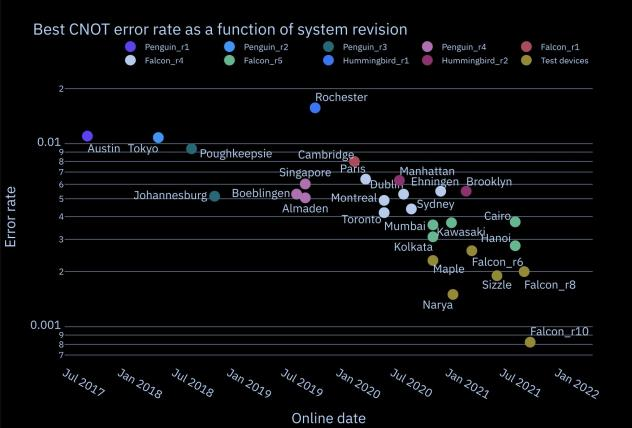
\includegraphics[scale=0.4]{cnot_ibm.jpg}\\
		{\scriptsize  https://twitter.com/jaygambetta/status/1445115380616335373 }
	\end{frame}

	\begin{frame}
		An alternative is use optimal quantum control.\\
		\vspace{.5cm}
		$\rightarrow$ Gradient Ascent Pulse Engineering (GRAPE) algorithm.\\
		\vspace{.5cm}
		Let us consider a system described by the Hamiltonian $H(t)=H(w(t))$, where $w(t)$ are continuous control parameters. GRAPE divides the temporal evolution into small temporal pieces with constant control parameters,
		\begin{equation*}
			H(t_k) = H_k(w_k).
		\end{equation*}
		
	\end{frame}

	\begin{frame}
		Then, considering a time step $\Delta t_k$, we have that the evolution piece is 
		\begin{equation*}
			U_k(w_k) = e^{-iH_k(w_k)\Delta t_k }.
		\end{equation*}
		After $N$ time steps, the total evolution is
		\begin{equation*}
			U(t_k,\vec{w}) = U_k(w_k)U_{k-1}(w_{k-1})\cdots U_1(w_1)U_{0}(w_{0}),
		\end{equation*}
		where $\vec{w}$ is a vector with the control parameters.
		
		\centering
		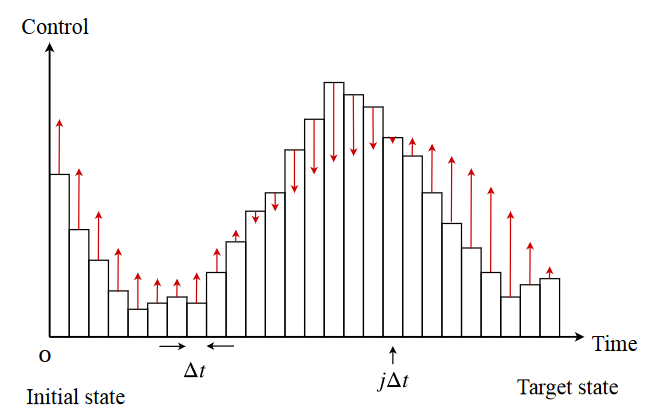
\includegraphics[scale=0.5]{grape}\\
		
		{\scriptsize  
			Y. Shi \emph{et al.}, "Optimized Compilation of Aggregated Instructions for Realistic Quantum Computers".}
		
	\end{frame}


	\begin{frame}
		In order to find the optimal control parameters we minimize numerically the fidelity with respect to the target gate $V$,
		
		\begin{equation*}
			f(\vec{w}) = \frac{1}{d^2} |  Tr( V^\dagger U(t_k,\vec{w})  ) |^2.
		\end{equation*}
		
		The performance of this quantum control depends on the precision of the model. We call it \emph{ex-situ} quantum control.
	\end{frame}

	\begin{frame}
		We can consider an alternative quantum control where the fidelity is evaluated on the quantum device, so that there are no limitations due to errors in the modeling. We call it \emph{in-situ} quantum control or \emph{quantum feedback}.
		\centering
		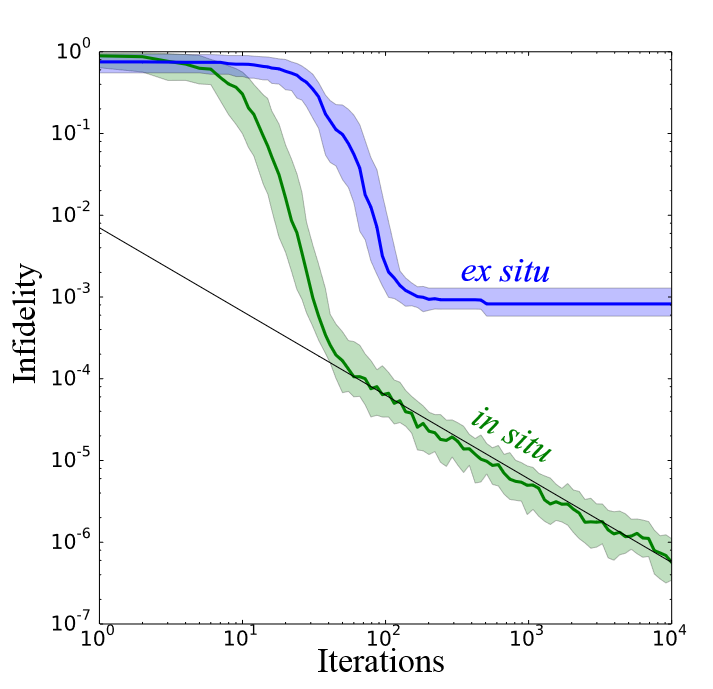
\includegraphics[scale=0.45]{fidelidad.png}\\
		
		{\scriptsize C. Ferrie and O. Moussa, "Robust and efficient in situ quantum control".}
	\end{frame}
	
	\begin{frame}
		There exist experimental techniques to evaluate the fidelity between an experimental gate and a theoretical gate.
		\vspace{0.3cm}
		\begin{itemize}
			\item Randomize benchmaking.
			\vspace{0.3cm}
			\item Direct fidelity estimation\\
			  {\scriptsize S. T. Flammia and Y.-K. Liu, "Direct Fidelity Estimation from Few Pauli Measurements".}
		\end{itemize}
	\end{frame}
	
	\begin{frame}
		\begin{itemize}
			\item Build a Qiskit library to perform the ex-situ and in-situ quantum control with GRAPE.\\
			\vspace{0.1cm}
			\item Propose a mixed protocol, where first the ex-situ quantum control is carried out, to then refine the result with in-situ quantum control.\\
			\vspace{0.1cm}
			\item Implement some relevant gate, such as c-not or toffoli.
		\end{itemize}
		
	\end{frame}
	
	\begin{frame}
		\centering
		
		Qiskit pulse has all the needed to carry out this project.
		
		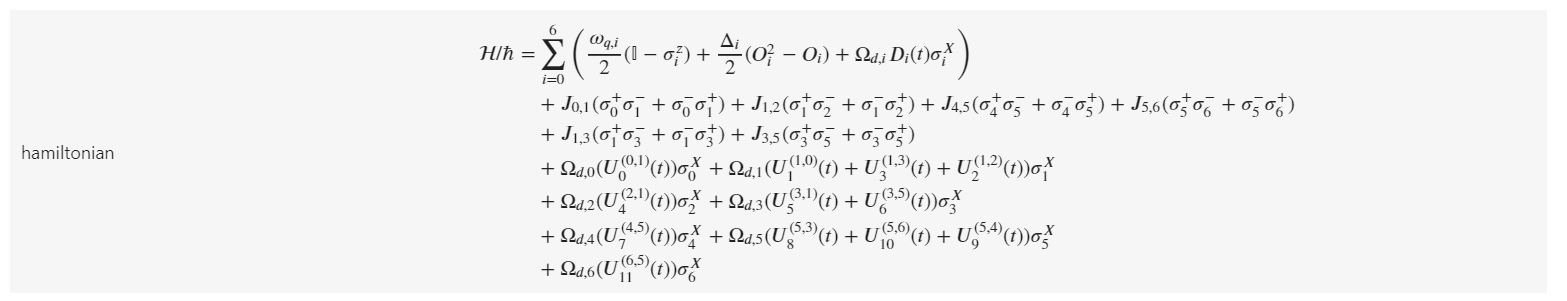
\includegraphics[scale=0.4]{hamiltonian_qiskit}
		
		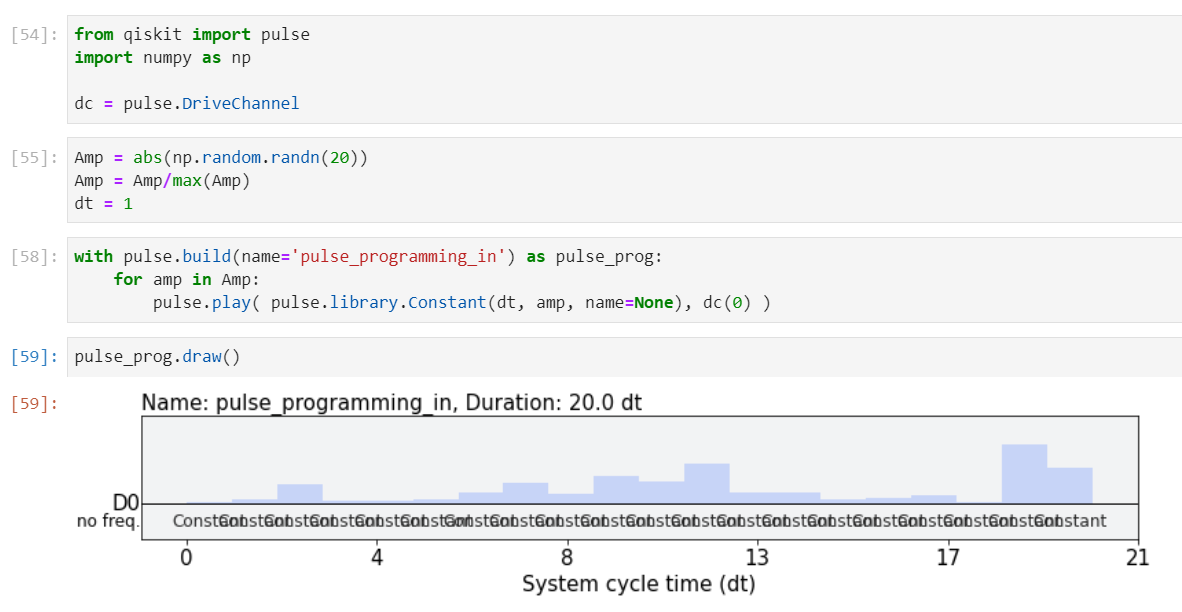
\includegraphics[scale=0.4]{grape_qiskit}
		
	\end{frame}
	
	
	\begin{frame}
		\centering
		Biggest challenge: evaluate the fidelity experimentally.
		
		I already have a module to measure the fidelity, but only between states. 
		
		We have to extend it to gates.
		
		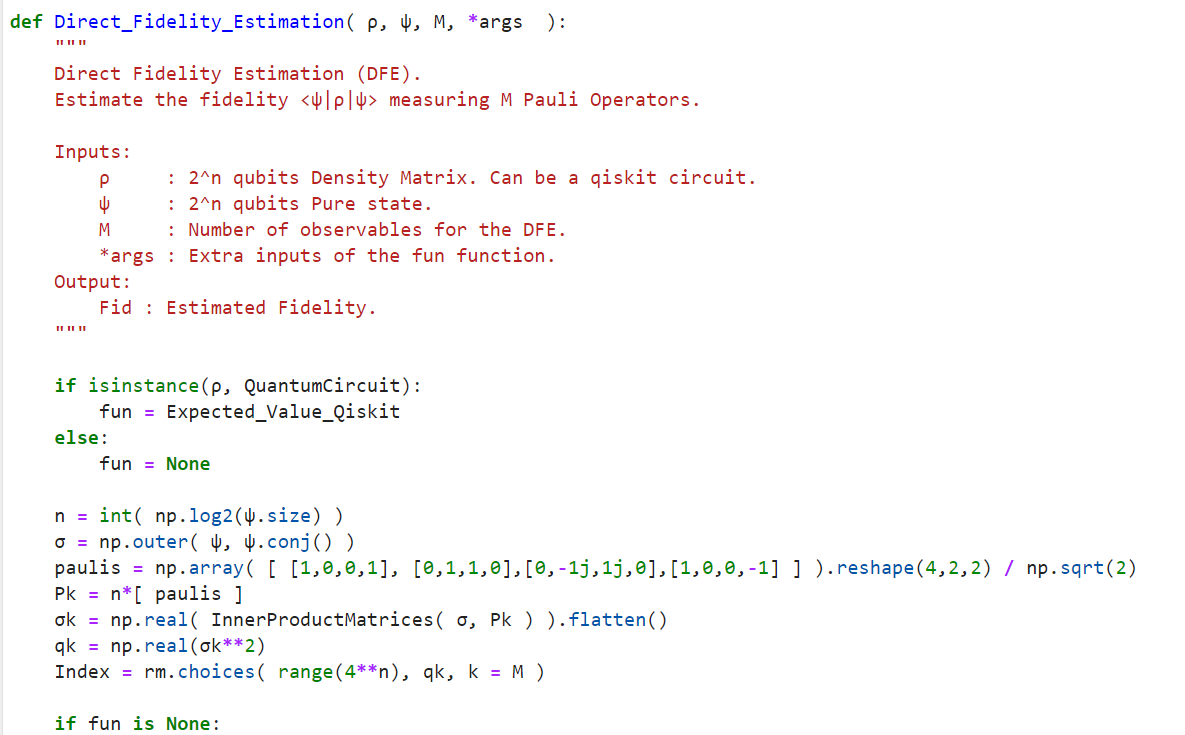
\includegraphics[scale=0.5]{direct_fidelity}
		
	\end{frame}
	
	
\end{document}















